\documentclass[tikz,border=10pt]{standalone}
\usetikzlibrary{arrows.meta, positioning, calc}
\usepackage[T1]{fontenc}
\usepackage{helvet}
\renewcommand{\familydefault}{\sfdefault}

\begin{document}
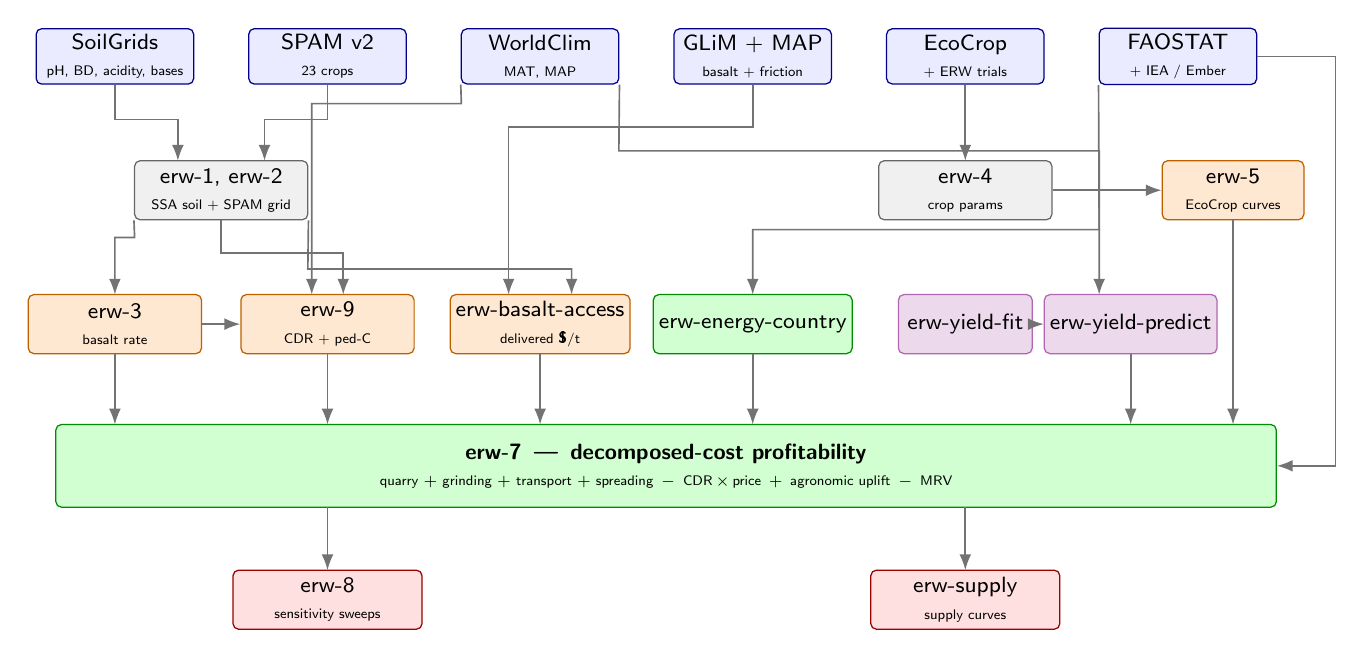
\begin{tikzpicture}[
  >=Latex,
  font=\sffamily\footnotesize,
  line width=0.45pt,
  every path/.append style={line cap=butt, line join=miter}
]

\tikzset{
  data/.style    ={draw=blue!55!black,   fill=blue!8,    rounded corners=2pt, minimum width=2.0cm, minimum height=0.70cm, align=center, inner sep=2pt},
  grid/.style    ={draw=black!60,        fill=gray!12,   rounded corners=2pt, minimum width=2.2cm, minimum height=0.75cm, align=center, inner sep=2pt},
  proc/.style    ={draw=orange!75!black, fill=orange!18, rounded corners=2pt, minimum width=2.2cm, minimum height=0.75cm, align=center, inner sep=2pt},
  bayes/.style   ={draw=violet!60,       fill=violet!15, rounded corners=2pt, minimum width=1.7cm, minimum height=0.75cm, align=center, inner sep=2pt},
  econ/.style    ={draw=green!55!black,  fill=green!18,  rounded corners=2pt, minimum width=2.4cm, minimum height=0.75cm, align=center, inner sep=2pt},
  outnode/.style ={draw=red!60!black,    fill=red!12,    rounded corners=2pt, minimum width=2.4cm, minimum height=0.75cm, align=center, inner sep=2pt},
  arr/.style     ={->, semithick, black!55}
}

% =========================================================
%   Nodes  (positions fixed so every arrow can be orthogonal)
% =========================================================

% --- Layer 0 : raw data sources ---
\node[data] (soil)  at ( 0.0, 6.2) {SoilGrids \\ {\tiny pH, BD, acidity, bases}};
\node[data] (spam)  at ( 2.7, 6.2) {SPAM v2 \\ {\tiny 23 crops}};
\node[data] (wclim) at ( 5.4, 6.2) {WorldClim \\ {\tiny MAT, MAP}};
\node[data] (glim)  at ( 8.1, 6.2) {GLiM + MAP \\ {\tiny basalt + friction}};
\node[data] (eco)   at (10.8, 6.2) {EcoCrop \\ {\tiny + ERW trials}};
\node[data] (fao)   at (13.5, 6.2) {FAOSTAT \\ {\tiny + IEA / Ember}};

% --- Layer 1 : working grid \& per-crop parameters ---
\node[grid] (wgrid)  at ( 1.35, 4.5) {erw-1, erw-2 \\ {\tiny SSA soil + SPAM grid}};
\node[grid] (cparam) at (10.80, 4.5) {erw-4 \\ {\tiny crop params}};
\node[proc, minimum width=1.8cm] (ecof) at (14.20, 4.5) {erw-5 \\ {\tiny EcoCrop curves}};

% --- Layer 2 : core geospatial surfaces ---
\node[proc]  (basalt) at ( 0.0, 2.8) {erw-3 \\ {\tiny basalt rate}};
\node[proc]  (cdr)    at ( 2.7, 2.8) {erw-9 \\ {\tiny CDR + ped-C}};
\node[proc]  (acc)    at ( 5.4, 2.8) {erw-basalt-access \\ {\tiny delivered \$/t}};
\node[econ]  (energy) at ( 8.1, 2.8) {erw-energy-country};
\node[bayes] (yfit)   at (10.8, 2.8) {erw-yield-fit};
\node[bayes, minimum width=2.0cm] (ypred) at (12.9, 2.8) {erw-yield-predict};

% --- Layer 3 : profitability convergence (wide so every surface drops straight) ---
\node[econ, minimum width=15.5cm, minimum height=1.05cm] (prof) at (7.0, 1.0)
  {\textbf{erw-7 \,---\, decomposed-cost profitability} \\
   {\tiny quarry $+$ grinding $+$ transport $+$ spreading \,$-$\, CDR\,$\times$\,price \,$+$\, agronomic uplift \,$-$\, MRV}};

% --- Layer 4 : downstream outputs ---
\node[outnode] (sens)   at ( 2.7, -0.7) {erw-8 \\ {\tiny sensitivity sweeps}};
\node[outnode] (supply) at (10.8, -0.7) {erw-supply \\ {\tiny supply curves}};

% =========================================================
%   Orthogonal arrows.  Every horizontal segment lives on a
%   dedicated y-track and every corner is a right angle.
%
%   Tracks above L1     :  5.4 (soil/spam fan-in)
%                          5.0 (wclim->ypred)
%                          5.3 (glim->acc)
%                          5.6 (wclim->cdr)
%   Tracks in L1-L2 gap :  4.0 (fao->energy)
%                          3.9 / 3.7 / 3.5 (wgrid fan-out)
%   Outside-right wrap  :  x = 15.0 (fao->prof)
% =========================================================

% ---------- Layer 0 -> Layer 1 ----------
% SoilGrids -> WGRID  (enters wgrid top, offset left of centre)
\draw[arr] (soil.south) -- (0.0, 5.4) -- (0.8, 5.4) -- (0.8, 4.875);
% SPAM -> WGRID  (enters wgrid top, offset right of centre)
\draw[arr] (spam.south) -- (2.7, 5.4) -- (1.9, 5.4) -- (1.9, 4.875);
% EcoCrop -> erw-4 crop-params  (same column - straight vertical)
\draw[arr] (eco.south)  -- (10.8, 4.875);

% ---------- Within Layer 1 ----------
\draw[arr] (cparam.east) -- (ecof.west);

% ---------- Layer 0 -> Layer 2  (skipping L1) ----------
% WorldClim -> erw-9 CDR    (south-west anchor, track y=5.6)
\draw[arr] (wclim.south west) -- (4.4, 5.6) -- (2.5, 5.6) -- (2.5, 3.175);
% WorldClim -> erw-yield-predict  (south-east anchor, track y=5.0)
\draw[arr] (wclim.south east) -- (6.4, 5.0) -- (12.5, 5.0) -- (12.5, 3.175);
% GLiM -> erw-basalt-access  (track y=5.3)
\draw[arr] (glim.south)       -- (8.1, 5.3) -- (5.0, 5.3) -- (5.0, 3.175);
% FAOSTAT (south-west) -> erw-energy-country  (drops below L1, track y=4.0)
\draw[arr] (fao.south west)   -- (12.5, 4.0) -- (8.1, 4.0) -- (8.1, 3.175);

% ---------- WGRID -> Layer 2  (three fans on three tracks) ----------
% WGRID (south-west) -> erw-3 basalt  (track y=3.9)
\draw[arr] (wgrid.south west) -- (0.25, 3.9) -- (0.0, 3.9) -- (0.0, 3.175);
% WGRID (south)      -> erw-9 cdr    (track y=3.7, enters cdr right of centre)
\draw[arr] (wgrid.south)      -- (1.35, 3.7) -- (2.9, 3.7) -- (2.9, 3.175);
% WGRID (south-east) -> erw-basalt-access  (track y=3.5, enters acc right of centre)
\draw[arr] (wgrid.south east) -- (2.45, 3.5) -- (5.8, 3.5) -- (5.8, 3.175);

% ---------- Within Layer 2 ----------
\draw[arr] (basalt.east) -- (cdr.west);
\draw[arr] (yfit.east)   -- (ypred.west);

% ---------- Layer 2 -> erw-7 (six straight drops to prof.north) ----------
\draw[arr] (basalt.south) -- (0.0,  1.525);
\draw[arr] (cdr.south)    -- (2.7,  1.525);
\draw[arr] (acc.south)    -- (5.4,  1.525);
\draw[arr] (energy.south) -- (8.1,  1.525);
\draw[arr] (ypred.south)  -- (12.9, 1.525);
% erw-5 EcoCrop-curves -> erw-7  (long drop at x=14.2, clear of ypred at x=12.9)
\draw[arr] (ecof.south)   -- (14.2, 1.525);

% ---------- FAOSTAT crop prices -> erw-7  (outside-right wrap) ----------
\draw[arr] (fao.east) -- (15.5, 6.2) -- (15.5, 1.0) -- (prof.east);

% ---------- erw-7 -> Layer 4 ----------
\draw[arr] (2.7,  0.475) -- (2.7,  -0.325);
\draw[arr] (10.8, 0.475) -- (10.8, -0.325);

\end{tikzpicture}
\end{document}
